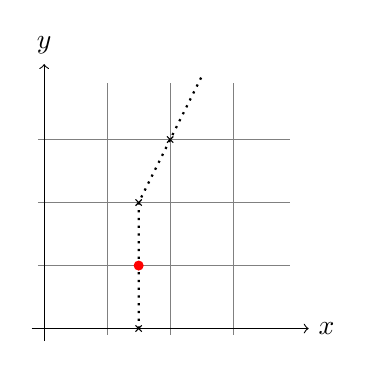
\begin{tikzpicture}[domain=0:4, scale=.8]
    \draw[very thin,color=gray] (-0.1,-0.1) grid (3.9,3.9);

    \draw[->] (-0.2,0) -- (4.2,0) node[right] {$x$};
    \draw[->] (0,-0.2) -- (0,4.2) node[above] {$y$};

    \draw[dotted, thick] (1.5,0) -- (1.5,2) -- (2.5,4);

    \draw[red] plot[only marks, mark=*] coordinates{(1.5,1)};
    \draw plot[only marks, mark=x] coordinates{(1.5,0) (1.5,2) (2,3)};
\end{tikzpicture}

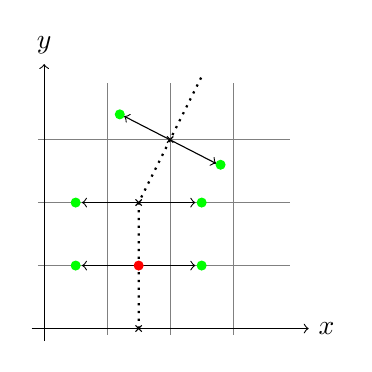
\begin{tikzpicture}[domain=0:4, scale=.8]
    \draw[very thin,color=gray] (-0.1,-0.1) grid (3.9,3.9);
    
    \draw[->] (-0.2,0) -- (4.2,0) node[right] {$x$};
    \draw[->] (0,-0.2) -- (0,4.2) node[above] {$y$};

    \draw[<->] (0.6, 1) -- (2.4, 1);
    \draw[<->] (0.6, 2) -- (2.4, 2);
    \draw[<->] (1.27, 3.37) -- (2.73, 2.62);
    
    \draw[dotted, thick] (1.5,0) -- (1.5,2) -- (2.5,4);
    
    \draw[red] plot[only marks, mark=*] coordinates{(1.5,1)};
    \draw plot[only marks, mark=x] coordinates{(1.5,0) (1.5,2) (2,3)};
    \draw[green] plot[only marks, mark=*] coordinates{(0.5,1) (2.5, 1) (0.5, 2) (2.5, 2) (1.2,3.4) (2.8, 2.6)};
    
\end{tikzpicture}



% \begin{tikzpicture}[domain=0:4]
%   \draw[very thin,color=gray] (-0.1,-0.1) grid (3.9,3.9);

%   \draw[->] (-0.2,0) -- (4.2,0) node[right] {$x$};
%   \draw[->] (0,-0.2) -- (0,4.2) node[above] {$y$};
%   \draw plot[only marks, mark=*] coordinates{(1,1)};
%   \draw[color=red]    plot (\x,\x)             node[right] {$f(x) =x$};
%   % \x r means to convert '\x' from degrees to _r_adians:
%   \draw[color=blue]   plot (\x,{sin(\x r)})    node[right] {$f(x) = \sin x$};
%   \draw[color=orange] plot (\x,{0.05*exp(\x)}) node[right] {$f(x) = \frac{1}{20} \mathrm e^x$};
% \end{tikzpicture}

